\chapter{TECNOLOGIAS EMPREGADAS}
\thispagestyle{empty}

Este capítulo apresenta um conceito simplificado sobre cada ferramenta utilizada para o desenvolvimento desta aplicação, ou que esteja diretamente relacionada a esta.


\section{Python}

Python é uma linguagem de programação poderosa, fácil de aprender de código aberto e livre. 

Ela possui estruturas eficientes e de alto nível de dados além de uma abordagem simples, entretanto eficaz, para programação orientada a objeto. Sua sintaxe elegante de tipagem dinâmica, juntamente com a sua natureza interpretável, tornam-na uma linguagem ideal para \textit{scripts} e desenvolvimento rápido de aplicações em muitas áreas, em diversas plataformas \cite{GUIDO}.

Por todas estas vantagens, hoje, Python é uma das linguagens mais utilizadas no mundo, assim muitas de suas bibliotecas e ferramentas são bem conhecidas. Abaixo serão descritas as ferramentas Buildout e Zope e a biblioteca Subprocess.


\subsection{Buildout}
\label{Buildout}

Buildout é uma ferramenta desenvolvida em Python, capaz de reproduzir o desenvolvimento de aplicações em um ambiente isolado. Ele fornece suporte para criação dessas aplicações, especialmente para as desenvolvidas Python. 

Esta ferramenta se baseia na execução de procedimentos especificado em um arquivo de configuração conhecido por \textit{recipe}

A partir de um conjunto de características e variáveis de ambiente previamente definidas nesse \textit{recipe}, é gerada a estrutura da aplicação, sendo esta composta pelas dependências de sistema,por pacotes Python ou mesmo por outras aplicações.

Um único \textit{recipe} de uma aplicação pode conter definições de configuração, processos e ainda outras aplicações, que por sua vez podem ser organizadas com seu próprio \textit{recipe} \cite{BRANDOM}.

Levando em consideração o ideal do ambiente isolado, também chamado de puro, a instalação do Buildout é extremamente simples podendo ser realizada a partir de um \textit{script} Python simples e de fácil acesso on-line, \cite{BOOTSTRAP}. Após executado, este \textit{script} gerará um segundo \textit{script} conhecido por ``bin/buildout''. 

Através do uso deste segundo \textit{script} é possível a execução das definições de cada \textit{recipe} a fim de obter a aplicação final. No exemplo \ref{xprompt} ocorre a construção da aplicação Xprompt.

{\singlespace
\begin{lstlisting}[caption=Exemplo de um \textit{script} Buildout,language=python,label={xprompt}]
[buildout]
develop = .
parts = 
  xprompt
  test

[xprompt]
recipe = zc.recipe.egg:scripts
eggs = xanalogica.tumbler
interpreter = xprompt

[test]
recipe = zc.recipe.testrunner
eggs = xanalogica.tumbler

\end{lstlisting}
}

O \textit{recipe} inicia-se com a declaração ``[Buildout]'', que é a única parte realmente obrigatória para identificá-lo como um \textit{recipe} do Buildout.

Caso a aplicação em questão esteja em desenvolvimento e/ou em fase de testes, utiliza-se a variável \textit{develop}, que deve informar a localização deste desenvolvimento.

Por \textit{parts} subentende-se o percurso do \textit{script}, isto é, a ordem de execução que o Buildout deve obedecer para instalação da aplicação independente da ordem que estejam descritas a aplicações ao longo do \textit{recipe}.

Cada \textit{part} possui uma descrição padrão que consiste de variáveis que envolvem cada componente responsável pela sua instalação. O \textit{eggs}, por exemplo, se trata da opção referente as dependências necessárias para execução desta parte.

O \textit{interpreter} é utilizado para gerar um interpretador Python contendo as dependências relacionadas em \textit{eggs}. Para utilizá-lo basta citá-lo e nomeá-lo. Neste caso o interpretador da aplicação será chamado ``xprompt''.

O tamanho de cada \textit{recipe} vária de acordo com a necessidade da aplicação. Neste caso com poucas especificações será possível gerar uma nova instância de uma aplicação Xprompt.

Ainda que incomum, é valido ressaltar que aplicações não necessariamente desenvolvidas em Python podem ter seu ambiente gerado pelo Buildout, com base na vasta disponibilidade de \textit{recipes} disponíveis. Isso geralmente é usado para suporte de dependências de sistema, em sua maioria desenvolvidas em C. O próprio Buildout será responsável por organizar e informar o caminho dessas aplicações, se necessário sobrescrevendo a variável de ambiente PATH.

\subsection{Subprocess}

O Subprocess é uma biblioteca Python que permite a criação de processos no sistema, similar a biblioteca Thread porém mais eficiente no quesito escalabilidade, pois permite que seus processos sejam divididos e utilizem diferentes processadores. 

Esta biblioteca foi criada na intenção de substituir outros módulos e funções obsoletas, e permitir também maior interação entre a aplicação e o sistema no qual se encontra.

{\singlespace
\begin{lstlisting}[caption=Exemplo de uso do Subprocess,language=python,label={codigo_subrocess}]
>>> import subprocess
>>> subprocess.Popen('echo "Hello World!"', shell=True)
Hello World!
\end{lstlisting}
}

No código \ref{codigo_subrocess} existe um pequeno exemplo de como o Subprocess pode ser utilizado.

Neste exemplo ele reproduz um acesso ao \textit{shell} do sistema a fim de demonstrar um \textit{Hello World} através do comando \textit{echo}, é possível observar o uso do \textit{shell} no final da segunda linha em que cita-se ``shell=True''.

Em aplicações que utilizam ambientes isolados, como citado na sessão \ref{Buildout}, é preferencial que a variável \textit{shell} tenha valor \textit{false},a fim de usar as aplicações deste ambiente, entretanto este já é seu valor por padrão, assim não é preciso declará-lo, como é visto no código \ref{codigo_subprocess_convert}.

Nesses casos também é preferível o uso da variável ``env'' que representa variáveis de \textit{environment}, isto é, variáveis de ambiente. Ao substituir esta variável o Buildout direciona o processo a utilizar os binários que estão no seu ambiente próprio ao invés do ambiente original, que neste caso é o próprio sistema.

O processo de sobrescrever a variável ``env'' é similar ao passo de redefinir a variável \textit{PATH} do sistema.

{\singlespace
\begin{lstlisting}[caption=Exemplo de uso do Subprocess com \textit{PIPE} extraído do CloudOoo,language=python,label={codigo_subprocess_convert}]
command = ["convert", self.file, output]
stdout, stderr = Popen(command, 
                        stdout=PIPE,
                        stderr=PIPE,
                        env=self.environment).communicate()
\end{lstlisting}
}


No exemplo, código \ref{codigo_subprocess_convert}, também é utilizada a opção \textit{PIPE} que permite ao comando Popen retornar as mensagens de saída e erro respectivamente através das variáveis \textit{stdout} e \textit{stderr}, para que seu conteúdo possa ser após o uso do comando.


\subsection{Zope}
\label{zope}

Zope (Z Object Publishing Environment) é um serviço web livre, de código aberto, desenvolvido em Python \cite{ZOPE2}, em outras palavras, um \textit{framework} Python.

Zope já foi considerado o principal responsável pela popularização do Python. Não existiu ferramenta em Perl que o levasse as pessoas como o Zope levou o Python \cite{UDELL}. Entretanto o Zope se tornou muito extenso e complexo, requerendo uma alta de taxa de aprendizagem e assim sendo ofuscado pela ferramenta Django em questão de popularidade.tanto

Dado seu nível de complexidade e todas as extensões disponíveis, muitos continuam utilizando o Zope, indiferentes a sua queda de popularidade, fazendo com que suas extensões continuem surgindo, sendo mantidas em processo de atualização continua por seus mantenedores.


\subsubsection{Zope Interfaces}

Como citado na sessão \ref{zope}, diversas extensões Zope foram desenvolvidas com intuito de auxiliar na criação de outras aplicações Python, de forma a não deixá-las muito extensas ou pesadas. Entre estas a \textit{zope.interface} é um exemplo de extensão independente escrita em Python e mantida pela equipe Zope.

A \textit{zope.interface} foi criada com intuito de permitir a comunicação entre quaisquer componentes externos que possuíssem uma \textit{Application Programming Interface} (API). A idéia de criar uma interface para os componentes de uma aplicação é uma forma  elegante de resolver um antigo problema de tipagem dinâmica tratando as informações recebidas de forma genérica, a fim de renderizá-las para um tratamento mais específico.


\section{XML}

\textit{Extensible Markup Language} (XML) é uma linguagem em formato de texto simples para representação de informações sobre estruturas, sejam elas de documentos, dados, configurações, entre outros. 

Esta linguagem foi derivada de um formato antigo chamado SGML, e adaptada para ser mais flexível ao uso Web \cite{W3C-XML}.

Atualmente se tornou um dos formatos mais comuns para compartilhamento de informações em aplicações web, por ter uma escrita simples e corresponder a um padrão similar ao HTML, que por muitos anos já vem sendo utilizado.

Além disso esta linguagem dispõe de outras vantagens como: padrão de \textit{markup}, cujo o nome é detalhado de forma redundante; a descrição da estrutura, que de forma geral também permite uma compreensão bem literal, como se fossem textos; todas suas versões são correspondentes, isto é, mesmo que algumas delas procurem por \textit{markups} específicos, qualquer versão mais nova de XML funcionará em uma aplicação que utilizasse uma versão anterior ou mais antiga.


\section{Formato Aberto}

O formato aberto é uma especificação publicada para armazenar dados digitais, mantido geralmente por uma organização de padrões não proprietária, e livre de limitações legais no uso.

Um formato aberto deve ser implementável tanto em software proprietário quanto em livre, usando as licenças típicas de cada um. Em oposição a esta idéia o formato proprietário é controlado e defendido por interesses particulares de empresas proprietárias detentoras de seus direitos.

O objetivo principal dos formatos abertos é garantir o acesso a longo prazo aos dados sem incertezas atuais ou futuras no que diz respeito às direitos legais ou à especificação técnica. Um objetivo secundário dos formatos abertos é permitir a competição de mercado, em vez de deixar que o controle de um distribuidor sobre um formato proprietário iniba o uso de um produto de competição.

\subsection{Formatos abertos de Documentos}
\label{documentos}

O \textit{.txt} é o formato aberto mais comum para arquivos de texto por ser pequeno e na maioria dos casos dispor de vários programas de edição em qualquer plataforma operacional, entretanto não é considerado o formato ideal para documentos, uma vez que não possui opções de formatação; tais como itálico e negrito.

Em 01 de maio de 2005, surgiu o \textit{OpenDocument Format}(ODF), um conjunto de formatos para aplicações de escritório com o objetivo de padronizar os formatos abertos para documentos. Seu nome original era \textit{Open Document Format for Office Application}, uma iniciativa da \textit{Organization for the Advancement of Structured Information Standards}(OASIS), baseado em um XML criado por desenvolvedores do OpenOffice.org. Esta aplicação na época era uma das poucas capazes de utilizar sua estrutura.

Atualmente os formatos ODF existem a 7 anos e foram adotados por diversas aplicações. Mesmo em sotwares proprietário entre elas o Microsoft Office, mesmo sendo um software originalmente proprietário através de um \textit{pluggin} ele permite a edição e manipulação destes formatos.

Através da figura \ref{crescimento_odf} é possível acompanhar o crescimento do uso do ODF até 2010, ano em que fez 5 anos.

\begin{figure}[ht]
    \centering
    \scalebox{0.7}{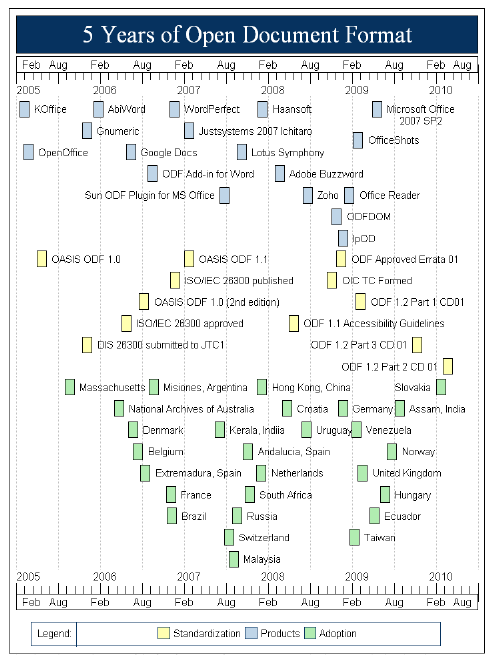
\includegraphics{figuras/crescimento_odf}}
    \caption{Crescimento do ODF nos primeiros cinco anos. Adaptado de \cite{SILVA}}
    \label{crescimento_odf}
\end{figure}

\begin{citacao}
O \textit{OpenDocument Format} ainda é uma incógnita à grande maioria dos usuários comuns, mas sua adoção cresce em várias partes do mundo, especialmente nos meios corporativos e governamentais. No Brasil, por exemplo, o ODF já conta inclusive com aprovação da Associação Brasileira de Normas Técnicas (ABNT), que aconteceu em 2008 (norma NBR ISO/IEC 26300)\cite{ALECRIM-ODF}.
\end{citacao}

\subsubsection{Formatos de documentos ODF}

O embora o mesmo padrão seja aplicado de forma geral em documentos ODF, esse padrão possui variações de extensões, no que diz respeito a documentos são elas:

\begin{itemize}
    \item{Para documentos de texto: .odt, .fodt;}
    \item{Para planilhas eletrônicas: .ods, .fods;}
    \item{Para apresentações: .odp, .fodp;}
    \item{Para bancos de dados: .odb;}
    \item{Para desenhos: .odg;}
    \item{Para fórmulas: .odf.}
\end{itemize}

E ainda existe um padrão a parte para modelos(\textit{templates}), são eles:

\begin{itemize}
    \item{Para documentos de texto: .ott;}
    \item{Para planilhas eletrônicas: .ots;}
    \item{Para apresentações: .otp;}
    \item{Para bancos de dados: .otb.}
\end{itemize}

Por guardar desde estrutura e dados textos até imagens presentes em seus arquivos a estrutura ODF é considerada um padrão comprimido assim como arquivo ZIP. É com base nesse padrão que diversas bibliotecas foram desenvolvidas para trabalhar com esses arquivos, entre elas a PyUno \ref{pyuno}.

\subsubsection{Estrutura de documentos ODF}

Como citado na sessão \ref{documentos} um documento ODF é uma estrutura de padrão aberto semelhante a arquivos comprimidos, como por exemplo arquivos ZIP.

Esta estrutura é composta principalmente por:

\begin{itemize}
    \item{mimetype: arquivo de linha única constituído pelo mimetype do documento;}
    \item{content.xml: arquivo que armazena o conteúdo criado pelo usuário do documento;}
    \item{meta.xml: arquivo responsável por armazenar os ``metadados'' do documento, ou seja, dados como autor, data de criação, data de modificação e outros;}
    \item{styles.xml: arquivo que contém os estilos do documento, tais como formatações de texto, parágrafos e outros;}
    \item{Pictures: pasta que armazena figuras existentes no documento.}
\end{itemize}

Existem ainda diversos arquivos e pastas que podem compor um documento ODF, mas que não são muito referidos em uso pratico.


\subsection{Formatos de Imagens}

No que diz respeito a imagens os formatos abertos tratam sobre patentes dos formatos, ou inclusa neles.

Assim em 1996 surgiu o formato \textit{Portable Network Graphics}(PNG) que tinha como principal objetivo substituir o formato GIF, portador de inúmeros algoritmos patenteados, que no entanto vieram a expirar em 2003.

Desde o princípio sua principal intenção foi sua utilização em qualquer aplicação sem necessidade de conflitos sobre patentes.

Além disso este formato permite comprimir imagens sem perda de qualidade e também a retirada do fundo de imagens através do canal alfa; possui suporte de milhões de cores, diferentemente do GIF, cujo suporte era de 256 cores; e ainda permite a criação de animações, cujas extensões podem variar em \textit{.mng} e \textit{.apng}, mas são igualmente livres.

Este formato é apoiado pela \textit{World Wide Web Consortium}(W3C), e se tornou um padrão internacional.

\subsubsection{Estrutura do PNG}

Um arquivo PNG consiste de uma assinatura PNG e seguido de vários blocos em serie \cite{PNG-BOOK}.

Sua assinatura equivale aos primeiros oito \textit{bytes}, consiste da serie “137 80 78 71 13 10 26 10”.

Cada bloco consiste de:

\begin{itemize}
    \item{length: inteiro correspondente ao numero de \textit{bytes} dos dados da imagem;}
    \item{chunk type: código equivalente ao tipo do bloco;}
    \item{chunk data: dados da imagem;}
    \item{Cyclic Redundancy Check(CRC): campo que contém o valor total de \textit{bytes} do bloco, o \textit{chunk type} e o \textit{chunk data}, mas sem o valor do \textit{length}.}
\end{itemize}

O inicio da serie de blocos deve conter um \textit{IHDR chunk} e o ultimo bloco deve conter um \textit{IEND chunk} como \textit{chunk type} sinalizando que representam o inicio e fim da serie respectivamente.

\subsubsection{Exif}

O \textit{Exchangeable Image File Format}(Exif) é um conjunto de ``metadados'' a respeito da imagem em questão, ou seja, são dados como autor, dia em que a foto foi tirada, câmera utilizada, entre outros listados conforme um padrão.

Todas essas informações ficam dentro da própria imagem, no entanto é preciso ter uma aplicação especifica para vê-lo, e em casos de informações mais abrangentes, as vezes é necessário possuir também uma aplicação para manipular a imagem e inserir nela ``metadados'' a respeito da imagem, aplicações estas como \ref{imagemagick}.

\subsection{Formatos de Áudio}

Os formatos abertos de áudio tratam sobre codecs disponíveis sem uma patente aplicada aos mesmos. Nesta categoria conta-se com os formatos Vorbis(.ogg) e \textit{Free lossless Áudio Codec}(.flac).

O .flac é um formato livre de áudio comprimível e sem perda de qualidade e dados durante a o processo de compreensão. Seu algoritmo permite que o arquivo reduza em até 60\% seu tamanho original, e também permite a manipulação de ``metadados''.

O .ogg é um novo formato comprimível de áudio. 
É comparado de forma grosseira com outros formatos utilizados para guardar e reproduzir musicas, tais como MP3, VQF, AAC, e outros formatos de áudio digital. Mas é diferente de todos estes formatos porque é livre, aberto e sem patentes \cite{XIPH}.

\subsection{Formatos de Vídeo}

Assim como os arquivos de áudio, a licença dos formatos de vídeo tratam sobre patentes de codecs, e neste caso as extensões mais comuns são conhecidas por Theora(.ogv) e Matroska(.mkv).

Theora é de propósito geral, um codec de vídeo com perda de dados. É baseado no codec de vídeo VP3 produzido pela \textit{On2 Tecnologies} \cite{XIPH-THEORA}.

Matroska é o nome de uma iniciativa ousada para a criação de formatos universais de \textit{containers} de áudio e vídeo digitais integrados, também chamados de formato de vídeo \cite{WIKIPEDIA-MATROSKA}.

Assim o .mkv trata-se de um ``contentor'' de padrão aberto para vídeos, que pode conter vários dados de diferentes tipos de codificações.

\section{LibreOffice}

O LibreOffice é um pacote de software, ou seja, uma suíte para documentos de escritório, de produtividade compatível com a maioria dos pacotes semelhantes, e que esta disponível para várias plataformas. É um software de código aberto, livre para baixar, utilizar e distribuir \cite{LibreOffice}.

Seu inicio foi marcado em 2000, quando a Sun Microsystems liberou o código de seu produto StarOffice. Neste momento se chamava OpenOffice.Org. 

Em 2010 a comunidade que desenvolvia o projeto anunciou uma fundação independente, \textit{The Document Foundation}, a fim de cumprir com a independência explicita da carta anunciada ao inicio do projeto.

Assim no inicio de 2011 foi lançado o LibreOffice 3.3, que bem como o OpenOffice.org 2.0, já suportava a edição da suíte \textit{OpenDocument}.


\subsection{UNO}
\label{uno}

O projeto LibreOffice possuía uma característica muito útil e pouco utilizada que era a capacidade de integrar seu funcionamento com outros aplicativos, isto é, um componente foi disponibilizada a fim de que aplicações em outras linguagens que estivessem fora do projeto pudessem interagir com o mesmo. Esse componente é conhecido por UNO (Universal Network Objects), que por sua vez é composto por um modelo dos componentes do LibreOffice.

O UNO oferece interoperabilidade entre diferentes linguagens de programação, diferentes modelos de objetos, diferentes arquiteturas e processos, em uma rede local ou mesmo através da internet. Seus componentes podem ser implementados e acessados através de \textit{bindings} deste \cite{MINETTO-PYUNO}.

Atualmente existem \textit{bindings} para as linguagens C, C++, Java e Python. Desde a versão 1.1 o LibreOffice dispõe do PyUNO em suas instalações por padrão.

\subsubsection{PyUNO}
\label{pyuno}

O PyUNO representa uma ``ponte'' entre o LibreOffice e aplicações Python. Através dele é possível a manipulação do componente UNO, seção \ref{uno}, para utilizar praticamente todas funcionalidades disponíveis no LibreOffice por \textit{scripts} Python.

No entanto, segundo \cite{PYUNO}, essa ferramenta ainda não atingiu seu uso absoluto podendo conter diversos \textit{bugs}, erros, e assim dependendo em grande parte de colaboração por parte da comunidade que utiliza a mesma.

No código \ref{example_uno} é possível ver um exemplo pratico do uso do PyUNO em um código Python:

{\singlespace
\begin{lstlisting}[caption=Exemplo de uso do Uno,language=python,label={example_uno}]
import sys
import os
import uno

# Get the uno component context from the PyUNO runtime
uno_context = uno.getComponentContext()
# Create the UnoUrlResolver on the Python side.
url_resolver = "com.sun.star.bridge.UnoUrlResolver"
resolver = uno_context.ServiceManager.createInstanceWithContext(
  url_resolver,
  uno_context)
# Connect to the running OpenOffice.org and get its context.
uno_connection = resolver.resolve("uno:socket,host=%s,port=%s;urp;StarOffice.ComponentContext" % (host, port))
# Get the ServiceManager object
return uno_connection.ServiceManager
\end{lstlisting}
}

Neste exemplo extraído diretamente do CloudOoo utiliza-se o contexto do processo ativo do PyUNO para retorna um serviço de gerenciamento do UNO, isto é, uma conexão é estabelecida entre o principal serviço de gerenciamento do UNO e o PyUNO utilizado pelo CloudOoo para que este possa por fim controlar as ações deste serviço.


\section{ImageMagick}
\label{imagemagick}

ImageMagick é uma suíte de aplicações para criar, editar,compor ou converter imagens \textit{bitmap} \cite{IMAGEMAGICK-STUDIO}.
Na realidade o ImageMagick disponibiliza um conjunto de binários, compatíveis com varias plataformas, que no Linux são dados como comandos de níveis, separados para diversas funcionalidades.

Para \cite{TESLA} é uma ferramenta, originalmente criada por John Cristy, para visualizar e manipular imagens, que esta amplamente disponível na Internet.

As funcionalidades que podem ser consideradas mais comuns e utilizadas são \textit{convert} e \textit{identify}, essas funcionalidades podem respectivamente: converter imagens para outros formatos ou formatação, como invertido ou de girar em 180 graus; e identificar os ``metadados'' disponíveis na imagem, como autor, ou data que foi criada ou tirada.

Como as demais ferramentas citadas por este trabalho, é um \textit{software} livre, disponível para baixar e utilizar da forma desejada ao usuário.


\section{XPDF}

Xpdf é uma suíte de binários de código aberto para visualização e manipulação básica de FFMPEG arquivos \textit{Portable Document Format}(PDF), criada por Glyph e Cog \cite{GLYPH-COG}.

Além de permitir a visualização de arquivos PDF o XPDF é uma ferramenta que permite a extração de textos dentro de documentos PDF e a conversão dos mesmos para o formato \textit{postscript}, formato este especialmente composto de informações e desenvolvido originalmente pela \textit{Adobe System}.

Assim como a maioria das aplicações para Linux é utilizada através de comandos, neste caso o mais comum \textit{pdftotext} o qual captura o texto disponível no documento PDF e retorna este texto através de um arquivo de texto simples.


\subsection{Poppler}

O poppler é uma biblioteca para renderizar PDF baseada no xpdf 3.0 \cite{JOHNSON}.

É uma das bibliotecas de código livre mais utilizada pelos sistemas Linux para leitores PDF, seu desenvolvimento é idealizado pela FreeDesktop.Org.


\section{PDFTk}

Se um documento PDF é um trabalho eletrônico, então o PDFTk é utilizado de removedor de grampos, furador, pasta, entre outros utilitários de documentos. o PDFTk é uma ferramenta consideravelmente simples para fazer as tarefas diárias com documentos PDF \cite{STEWARD}.

Esta ferramenta esta sob licença GPL e utiliza bibliotecas que possuem suas próprias licenças de uso.

Na realidade de simples o PDFTk tem apenas sua forma de uso, pois realiza tarefas complicadas no contexto de documentos PDF. Sua confiabilidade é altamente elogiável dado que seu criador e principal mantenedor, Sid Steward, é também autor do livro “PDF Hacks”, que é considerado uma das referências do ramo.


\section{FFMPEG}

Para \cite{FFMPEG-SCALABLE}, a melhoria constante do uso do processamento de multimédia, requerida e obtida pela expansão multi funcional e acelerada dos equipamentos de hardware, requer também aplicações eficientes e escaláveis a medida que este processo avança. E partindo deste principio uma das ferramentas ideais para projetos escaláveis é o FFMPEG.

FFMPEG é um rápido conversor de vídeo e áudio que também consegue tratar informações de ambos. Ele é capaz de converter faixas arbitrarias de amostras e redimensionar vídeos através de filtros polifásicos de alta qualidade \cite{FFMPEG}.

Mais do que isso, o FFMPEG é uma suíte de aplicações via linha de comando capaz de converter, extrair e inserir ``metadados'' em arquivos de áudio e vídeo de simples entendimento, de fácil uso.


\section{SERVIÇOS WEB}

Segundo \cite{PIRNAU}, os serviços web representam a metodologia em que aplicações podem se comunicar através de mensagens assíncronas ou chamadas remotas. Assim pode se dizer que serviços web são aplicações acessáveis remotamente.

Toda empresa tem por objetivo prover serviços, sejam esses para própria empresa, ou para clientes que por sua podem ser outras empresas. A anos esses serviços têm sido automatizados, inicialmente aplicações \textit{desktop} eram criadas quando a empresa era pequena e possuía poucas maquinas, ou a comunicação entre elas não era tão necessária.

Quando a rede passou a estar presente no dia a dia de forma geral essas aplicações foram evoluindo e buscando a comunicação entre as mesmas.

Este conceito na verdade trata da iniciativa por parte dessas empresas de retirar suas aplicações da maquinas próprias e passá-las para potente servidores que disponibilizarão esta na internet, assim basta ter acesso a internet e é possível utilizar esta aplicação.


\section{XML-RPC}

É um protocolo para chamadas remotas que utiliza HTTP para transporte e XML para codificação. O XML-RPC foi desenhado para ser o mais simples o possível, enquanto permite que uma estrutura de dados complexa seja transmitida, processada e retornada \cite{XMLRPC}.

Foi originalmente criado por Dave Winer na \textit{UserLand Frontier}, e inspirado por outros dois protocolos, um deles também desenvolvido pelo próprio Dave Winer e outro que representava o começo do protocolo SOAP. Entretanto seu uso é bem mais simples de se utilizar e entender que o SOAP. Suas mensagens correspondem a uma requisição \textit{HTTP-POST}, enquanto composição do corpo da mensagem é escrita em XML, bem como a resposta que a requisição recebe.

Dada sua simplicidade e eficiência se tornou um protocolo muito popular e utilizado hoje nos dias atuais.


\section{WSGI}

O \textit{Web Service Gateway Interface}(WSGI) é uma interface de entrada de dados para serviços web. É também uma especificação para que serviços e aplicações web se comuniquem com outras aplicações web, embora possa ainda ser utilizada para outras funções. É um padrão Python, escrito sob a \textit{PEP} 333 \cite{WSGI}.

Esta interface foi escrita com o objetivo de fornecer uma forma relativamente simples e compreensiva de comunicação entre aplicações e servidores, ou pelo menos com a maioria das aplicações web em Python, e que ainda pudesse suportar componentes \textit{middleware}.


\subsection{Paster}

Paster se trata de um componente para serviços web, composto pelo Python \textit{Paste}, que segue o padrão da interface Python WSGI.

Possui dois níveis de linha de comando composto inicialmente por \textit{paster}, onde o segundo comando especifica o serviço desejado, como \textit{serve} no caso de estabelecer o servidor, seguindo como parâmetros o restante das informações necessárias para estabelecer o serviço desejado.

É considerado um dos mais simples servidores web para Python, no entanto pode ser utilizado assincronamente e manter uma escalabilidade considerável até 2000\textit{rps}.


\section{Git}

Git é um sistema de controle de versões distribuídas livre e de código aberto, projetado para lidar com qualquer projeto, desde o menor ao maior com rapidez e eficiência \cite{SOFTWARE-FREEDOM-CONSERVANCY}.

A historia do Git está muito relacionada a criação do Linux e de Linus Torvalds, seu criador, bem como com toda comunidade de desenvolvimento Linux. Durante anos a comunidade utilizou a ferramenta \textit{BitKeeper} para guardar a modificações do projeto.

Em 2005, após um problema com a proprietária deste, a comunidade decidiu criar sua própria ferramenta a partir da experiência com a anterior, houve um novo foco em: velocidade, \textit{design} simples, suporte para desenvolvimento paralelo, distribuição completa e a habilidade necessária para lidar com projetos grandes sem perda de velocidade e dados.

Assim, esse novo sistema de versionamento permite que qualquer repositório seja o centro do versionamento, deixando todo \textit{log} das modificações guardados nele sem que para isso precise de uma conexão a rede ou servidor geral.


\subsection{Git e Subversion}

Diferentemente do Git, o Subversion é um sistema de controle de versões centralizado, entretanto muito utilizado atualmente, principalmente por projetos livres.

Embora seja consideravelmente rápido, é extremamente desaconselhável para projetos grandes e principalmente desenvolvidos paralelamente.
